\begin{figure}[ht]
\centering
% Thesis-wide categorical color palette
% Usage: % Thesis-wide categorical color palette
% Usage: % Thesis-wide categorical color palette
% Usage: \input{figures/palette} in any figure file
%
% Muted primary colors -- print-friendly, visually distinct.
% Inspired by Cooper Union's red/blue primaries, softened for
% academic figures. Use palA-palC for data series in scatter
% plots, line charts, bar charts, etc.

\definecolor{palA}{HTML}{1F77B4}   % Tableau blue
\definecolor{palB}{HTML}{D62728}   % Tableau red
\definecolor{palC}{HTML}{2CA02C}   % Tableau green
 in any figure file
%
% Muted primary colors -- print-friendly, visually distinct.
% Inspired by Cooper Union's red/blue primaries, softened for
% academic figures. Use palA-palC for data series in scatter
% plots, line charts, bar charts, etc.

\definecolor{palA}{HTML}{1F77B4}   % Tableau blue
\definecolor{palB}{HTML}{D62728}   % Tableau red
\definecolor{palC}{HTML}{2CA02C}   % Tableau green
 in any figure file
%
% Muted primary colors -- print-friendly, visually distinct.
% Inspired by Cooper Union's red/blue primaries, softened for
% academic figures. Use palA-palC for data series in scatter
% plots, line charts, bar charts, etc.

\definecolor{palA}{HTML}{1F77B4}   % Tableau blue
\definecolor{palB}{HTML}{D62728}   % Tableau red
\definecolor{palC}{HTML}{2CA02C}   % Tableau green

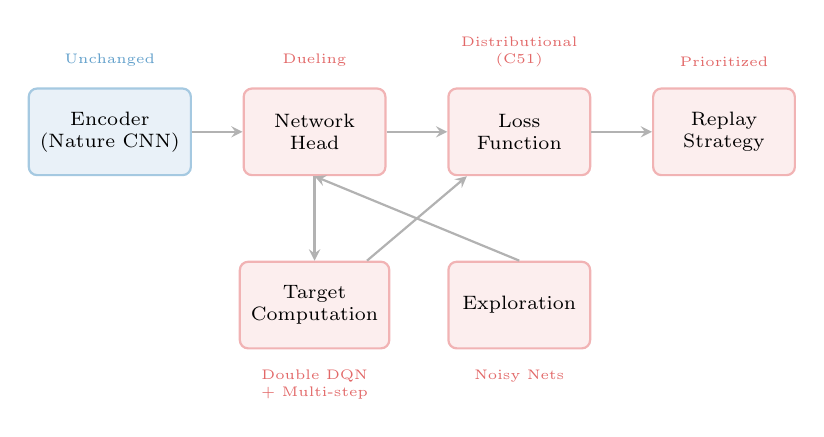
\begin{tikzpicture}[
    comp/.style={draw=black!30, thick, rounded corners=3pt,
                 minimum width=1.8cm, minimum height=1.1cm,
                 font=\scriptsize, align=center, inner sep=4pt},
    unchanged/.style={comp, fill=palA!10, draw=palA!40},
    changed/.style={comp, fill=palB!8, draw=palB!35},
    arr/.style={->, thick, >=stealth, black!30},
    ext/.style={font=\tiny, text=palB!70, align=center},
    ulbl/.style={font=\tiny, text=palA!70},
]

% Components (left to right flow)
\node[unchanged] (enc) at (0, 0) {Encoder\\(Nature CNN)};
\node[changed]   (head) at (2.6, 0) {Network\\Head};
\node[changed]   (loss) at (5.2, 0) {Loss\\Function};
\node[changed]   (replay) at (7.8, 0) {Replay\\Strategy};

% Second row
\node[changed]   (target) at (2.6, -2.2) {Target\\Computation};
\node[changed]   (explore) at (5.2, -2.2) {Exploration};

% Arrows
\draw[arr] (enc) -- (head);
\draw[arr] (head) -- (loss);
\draw[arr] (loss) -- (replay);
\draw[arr] (head) -- (target);
\draw[arr] (target) -- (loss);
\draw[arr] (explore.north) -- (head.south);

% Extension labels
\node[ext, above=4pt] at (head.north)  {Dueling};
\node[ext, above=4pt] at (loss.north)  {Distributional\\(C51)};
\node[ext, above=4pt] at (replay.north) {Prioritized};
\node[ext, below=4pt] at (target.south)
    {Double DQN\\+ Multi-step};
\node[ext, below=4pt] at (explore.south) {Noisy Nets};

% Unchanged label
\node[ulbl, above=4pt] at (enc.north) {Unchanged};

\end{tikzpicture}
\caption{Rainbow modifies five of six DQN components. The
  convolutional encoder -- where SPR operates -- is the only
  component left unchanged.}
\label{fig:rainbow-components}
\end{figure}
